\documentclass[tikz]{standalone}
\usepackage{tikz,pgfplots,amssymb}
\usepgfplotslibrary{fillbetween}
% \usetikzlibrary{fillbetween}
% \usepgfplotslibrary{decorations.softclip}

\begin{document}
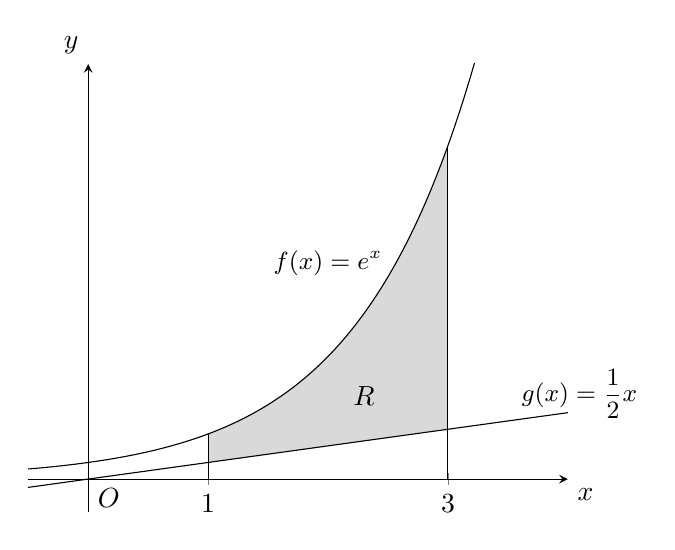
\begin{tikzpicture}[>=stealth]
\begin{axis}[
axis x line=center,
axis y line=center,
xlabel={$x$},
ylabel={$y$},
xtick={1,3},
ytick={.},
xlabel style={below right},
ylabel style={above left},
xmin=-0.5,
xmax=4,
ymin=-2,
ymax=25
]

\addplot [mark=none, domain=-0.5:4, samples=201, name path=f] {e^x};
\addplot [mark=none, domain=-0.5:4, samples=201, name path=l] {x};

\addplot[gray!30] fill between[of=f and l, soft clip={(axis cs:1, 0) rectangle (axis cs:3, e^3)}];
\node at (axis cs:2.3,5) {$R$};
\node[below right] at (axis cs:0,0) {$O$};

\node at (axis cs:2,13) {\small $f(x)=e^x$};

% \draw (axis cs:1, 0) -- (axis, cs:1, e^1);
% \draw (axis cs:3, 0) -- (axis, cs:3, e^3);
% https://tex.stackexchange.com/questions/170664/foreach-not-behaving-in-axis-environment
% \pgfplotsinvokeforeach{0.00,0.1,...,1.00}{
%     \draw [red] (axis cs:0,#1) -- (axis cs:1,#1);
% }
\foreach \xValue in {1,3} {
    \edef\temp{\noexpand\draw (axis cs:\xValue, 0) -- (axis cs:\xValue, e^\xValue);}
    \temp
}

\end{axis}

\node at (7,1.5) {\small $\displaystyle g(x)=\frac{1}{2}x$};

\end{tikzpicture}
\end{document}
